% This is text associated with the open textbook "Open Electromagnetics"
% See immediately below for author, date
% This work is licensed under the Creative Commons Attribution-ShareAlike 4.0 International License. (CC BY-SA 4.0) 
% To view a copy of the license, visit http://creativecommons.org/licenses/by-sa/4.0/

%ORB TITLE Single-Stub Matching
%ORB AUTHOR 0        # S.W. Ellingson, Virginia Tech (ellingson@vt.edu)
%ORB DATE 20180802   # yyyymmdd
%ORB ABSTRACT Single-stub matching.  Refers explicitly to module m0093 (single-reactance matching)

\label{m0094_Single-Stub_Matching} % <-- Must match name of this file and module directory name.  Don't mess with this!
\index{stub!applications|(}
\index{impedance!matching|(}
\index{single-stub matching|(}

In Section~\ref{m00093_Single-Reactance_Matching}, we considered impedance matching schemes consisting of a transmission line combined with a reactance which is placed either in series or in parallel with the transmission line.  
In many problems, the required discrete reactance is not practical because it is not a standard value, or because of non-ideal behavior at the desired frequency (see Section~\ref{m0092_Impedance_Matching_General_Considerations} for more about this), or because one might simply wish to avoid the cost and logistical issues associated with an additional component.
Whatever the reason, a possible solution is to replace the discrete reactance with a transmission line ``stub'' -- that is, a transmission line which has been open- or short-circuited.
Section~\ref{m0088_Input_Impedance_for_Open_and_Short_Circuit_Terminations} explains how a stub can replace a discrete reactance.  
Figure~\ref{m0094_fSSM-SMA} shows a practical implementation of this idea implemented in microstrip.  This section explains the theory, and we'll return to this implementation at the end of the section.
%
\begin{figure}[b!]
\begin{center}
\pdftooltip{{  % note double braces
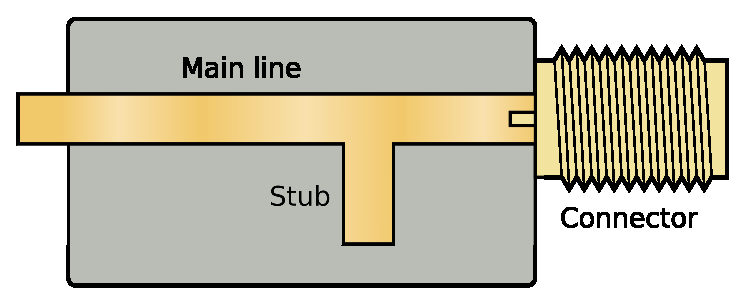
\includegraphics[width=\columnwidth]{modules/m0094_fSSM-SMA.eps}
% https://commons.wikimedia.org/wiki/File:Stripline_stub_matching.svg
}}{A gold-colored microstrip transmission line going through a gray rectangular field. The main line extends horizontally with an arrow inside it pointing to the left to indicate direction. A stub extends downwards perpendicularly from the main line within the gray field. The right end of the main line is capped by a threaded connector outside of the gray field.}
\end{center} 
\centerline{\scriptsize 
\hyperref[m0094_fSSM-SMA_Credit]{Spinningspark} 
\href{https://creativecommons.org/licenses/by-sa/3.0/deed.en}{CC BY~SA 3.0} 
} 
\caption{
\label{m0094_fSSM-SMA}
A practical implementation of a single-stub impedance match using microstrip transmission line.  Here, the stub is open-circuited.
}
\end{figure}

Figure~\ref{m0094_fSSM} shows the scheme.
This scheme is usually implemented using the parallel reactance approach, as depicted in the figure.
Although a series reactance scheme is also possible in principle, it is usually not as convenient.
This is because most transmission lines use one of their two conductors as a local datum; e.g., the ground plane of a printed circuit board for microstrip line is tied to ground, and the outer conductor (``shield'') of a coaxial cable is usually tied to ground.
This is contrast to a discrete reactance (such as a capacitor or inductor), which does not require that either of its terminals be tied to ground.  
This issue is avoided in the parallel-attached stub because the parallel-attached stub and the transmission line to which it is attached \emph{both} have one terminal at ground.
%
\begin{figure}
\begin{center}
\pdftooltip{{  % note double braces
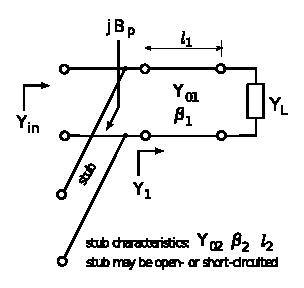
\includegraphics[width=2.5in]{modules/m0094_fSSM.eps}
}}{A transmission line with three nodes on both the input and output branches. Starting at the top left and going clockwise, a stub extending perpendicularly from the input and output terminals is connected between the source terminal and the middle terminal. The length between the middle terminal and the impedance terminal is measured l sub 1. Y sub 01 is measured across the terminals on either side of the impedance, with beta sub 1 underneath. The impedance is labeled Y sub L. An arrow pointed toward the impedance at the middle terminal on the bottom side is labeled Y sub 1. Underneath the graphic are the words "stub characteristics: Y sub 02, beta sub 2, l sub " and "stub may be open- or short-circuited".}
\end{center} 
\caption{\label{m0094_fSSM}Single-stub matching.}
\end{figure}

The single-stub matching procedure is essentially the same as the single parallel reactance method, except the parallel reactance is implemented using a short- or open-circuited stub as opposed a discrete inductor or capacitor.  Since parallel reactance matching is most easily done using admittances, 
\label{admittance}
it is useful to express Equations~\ref{m0088_eZstubSC} and \ref{m0088_eZstubOC} (input impedance of an open- and short-circuited stub, respectively, from Section~\ref{m0088_Input_Impedance_for_Open_and_Short_Circuit_Terminations}) in terms of susceptance:
\index{susceptance}
%
\begin{equation}
B_p = -Y_{02} \cot\left(\beta_2 l_2\right) ~~\mbox{short-circuited stub}
\end{equation}
%
\begin{equation}
B_p = +Y_{02} \tan\left(\beta_2 l_2\right) ~~\mbox{open-circuited stub}
\end{equation}
%
As in the main line, the characteristic impedance $Z_{02}=1/Y_{02}$ is an independent variable and is chosen for convenience.

A final question is when should you use a short-circuited stub, and when should you use an open-circuited stub?
Given no other basis for selection, the termination that yields the shortest stub is chosen.
An example of an ``other basis for selection'' that frequently comes up is whether DC might be present on the line. If DC is present with the signal of interest, then a short circuit termination without some kind of remediation to prevent a short circuit for DC would certainly be a bad idea.

In the following example we address the same problem raised in Section~\ref{m00093_Single-Reactance_Matching} (Examples~\ref{m0093_eSSR-S} and \ref{m0093_eSSR-P}), now using the single-stub approach:
~\\
%
%ORB EXAMPLE
~\\ \begin{example} 
\begin{mdframed}[backgroundcolor=brown!20,linecolor=brown!20]\raggedright
Single stub matching.
\\~\\
% This is from HW9 of ECE3106 15Fa
Design a single-stub match that matches a source impedance of $50\Omega$ to a load impedance of $33.9 + j17.6~\Omega$. %at 1.5~GHz. 
Use transmission lines having characteristic impedances of $50\Omega$ throughout, and leave your answer in terms of wavelengths.

{\bf Solution.}
From the problem statement: $Z_{in} \triangleq Z_S = 50~\Omega$ and $Z_L = 33.9+j17.6~\Omega$ are the source and load impedances respectively.
$Z_0=50~\Omega$ is the characteristic impedance of the transmission lines to be used.
The reflection coefficient $\Gamma$ (i.e., $Z_L$ with respect to the characteristic impedance of the transmission line) is
%
\begin{equation}
\Gamma \triangleq \frac{Z_L - Z_0}{Z_L + Z_0} \cong -0.142 + j0.239
\end{equation} 
%
The length $l_1$ of the primary line (that is, the one that connects the two ports of the matching structure) is the solution to the equation (from Section~\ref{m00093_Single-Reactance_Matching}):
%
\begin{equation}
\mbox{Re}\left\{Y_1\right\} = \mbox{Re}\left\{Y_{01} \frac{ 1 - \Gamma e^{-j2\beta_1 l_1} }{ 1 + \Gamma e^{-j2\beta_1 l_1} }\right\}
\end{equation}
% 
where here
$\mbox{Re}\left\{Y_1\right\}=\mbox{Re}\left\{1/Z_S\right\}=0.02$~mho and 
$Y_{01} = 1/Z_0 = 0.02$~mho.
Also note
%
\begin{equation}
2\beta_1 l_1 = 2 \left(\frac{2\pi}{\lambda}\right) l_1 = 4\pi \frac{l_1}{\lambda}
\end{equation}
%
where $\lambda$ is the wavelength in the transmission line.
So the equation to be solved for $l_1$ is:
%
\begin{equation}
1 = \mbox{Re}\left\{ 
           \frac{ 1-\Gamma e^{-j4\pi l_1/\lambda } }
                { 1+\Gamma e^{-j4\pi l_1/\lambda } } \right\} 
\end{equation}
%
By trial and error (or using the Smith chart; see ``Additional Reading'' at the end of this section) we find \underline{$l_1\cong 0.020\lambda$} for the primary line, yielding $Y_1 \cong 0.0200-j0.0116$~mho for the input admittance after attaching the primary line.  

We now seek the shortest stub having an input admittance of $\cong +j0.0116$~mho to cancel the imaginary part of $Y_1$.  
For an open-circuited stub, we need
%
\begin{equation}
B_p = +Y_0 \tan{2\pi l_2/\lambda} \cong +j0.0116~\mbox{mho}
\end{equation}
%
The smallest value of $l_2$ for which this is true is $\cong 0.084\lambda$.  
For a short-circuited stub, we need
%
\begin{equation}
B_p = -Y_0 \cot{2\pi l_2/\lambda} \cong +j0.0116~\mbox{mho}
\end{equation}
%
The smallest positive value of $l_2$ for which this is true is $\cong 0.334\lambda$; i.e., much longer.  
Therefore, we choose the \underline{open-circuited stub} with \underline{$l_2\cong 0.084\lambda$}.  
Note the stub is attached in parallel at the source end of the primary line.

\end{mdframed}\end{example}

%Finally, returning to Figure~\ref{m0094_fSSM-SMA}, 
Single-stub matching is a very common method for impedance matching using microstrip lines at frequences in the UHF band (300-3000~MHz) and above.  In Figure~\ref{m0094_fSSM-SMA}, the top (visible) traces comprise one conductor, whereas the ground plane (underneath, so not visible) comprises the other conductor.  The end of the stub is not connected to the ground plane, so the termination is an open circuit.  A short circuit termination is accomplished by connecting the end of the stub to the ground plane using a \emph{via}; that is, a plated-through that electrically connects the top and bottom layers.

%%%%%%%%%%%%%%%%%%%%%%%%%%%%%%%%%%

{\bf Additional Reading:}
\begin{itemize}
\item ``\href{https://en.wikipedia.org/wiki/Stub_(electronics)}{Stub (electronics)}'' on Wikipedia.
\item ``\href{https://en.wikipedia.org/wiki/Smith_chart}{\small Smith chart}'' on Wikipedia.
\item ``\href{https://en.wikipedia.org/wiki/Via_(electronics)}{Via (electronics)}'' on Wikipedia.
\end{itemize}

\index{stub!applications|)}
\index{impedance!matching|)}
\index{single-stub matching|)}
